\documentclass{article}
\usepackage{url}
\usepackage{hyperref}
\usepackage{fullpage}
\usepackage{graphicx}
\usepackage{natbib}
\usepackage{amsmath}
\usepackage{color}

% BEAST book specific commands
\newcommand{\BEASTVersion}{2.4.x}
\newcommand{\TracerVersion}{1.6}
\newcommand{\FigTreeVersion}{1.4.2}

\newcommand{\chainLength}{{5,000,000}}
\newcommand{\logEvery}{{5,000}}
\newcommand{\screenEvery}{{10,000}}

\newcommand{\Conv}{\mathop{\scalebox{1.5}{$\ast$}}}

\setlength{\parskip}{1em}
\renewcommand{\baselinestretch}{1.5}

\begin{document}
\title{StarBEAST2 -- Species Trees with Relaxed Molecular Clocks}

\author{Joseph Heled, Remco Bouckaert, Walter Xie, Alexei J Drummond and Huw A Ogilvie}

\maketitle

\section{Introduction}

In this tutorial we demonstrate the use of StarBEAST2, a fully Bayesian method
of species tree estimation and a replacement for $\Conv$BEAST
\citep{Heled01032010}. StarBEAST2 is many times faster than $\Conv$BEAST,
and also supports applying a relaxed clock to the species tree. This enables
estimating the substitution rates of extant and ancestral species under a
multispecies coalescent model.

You will need to download and install the following software:

\begin{itemize}
\item \textbf{BEAST} - this package contains BEAST, BEAUti,
TreeAnnotator, DensiTree, and other programs. This tutorial is written
for BEAST 2 \citep{10.1371/journal.pcbi.1003537} version {\BEASTVersion}, which is available for download from
\url{http://beast2.org/}.
\item \textbf{Tracer} - this program is used to explore the output of BEAST (and
other Bayesian MCMC programs). It graphically and quantitively summarizes the
distributions of continuous parameters and provides diagnostic information. At
the time of writing, the current version is {\TracerVersion}, which is available
for download from \url{http://tree.bio.ed.ac.uk/software/tracer/}.
\item \textbf{FigTree} - this is an application for displaying and printing
molecular phylogenies, in particular those obtained using BEAST. At the time of
writing, the current version is {\FigTreeVersion}, which is available for download
from \url{http://tree.bio.ed.ac.uk/software/figtree/}.
\end{itemize}

\section{BEAST}

This tutorial will guide you through the analysis of seven loci sampled from 26
individuals representing eight species of pocket gophers, a data set which was
originally gathered and analysed by
\cite{belfiore2008multilocus}. The objective of this tutorial is to estimate the
species tree that is most probable given the multi-individual multi-locus
sequence data. The species tree has eight taxa, whereas each gene tree has 26
taxa. StarBEAST2 will co-estimate seven gene trees embedded in a shared species
tree \citep{Heled01032010}.

The first step will be to convert a NEXUS file with a DATA or CHARACTERS block
into a BEAST XML input file. This is done using the program BEAUti (Bayesian
Evolutionary Analysis Utility). This is a user-friendly program for setting the
evolutionary model and options for the MCMC analysis. The second step is to
actually run BEAST using the input file that contains the data, model and
settings. The final step is to explore the output of BEAST in order to diagnose
problems and to summarize the results.

\subsection*{BEAUti}

Run BEAUti by double clicking on its icon, or by launching the BEAUTi executable
file from the command line in Linux.

\subsubsection*{Set up BEAUti for StarBEAST2}

StarBEAST2 can be easily installed from within BEAUTi. First choose the
\textbf{File/Manage Packages} menu item, which will then display the list of
packages available for installation (Figure~\ref{fig:managePackages}). Select
the StarBEAST2 package and then install it by clicking the
\textbf{Install/Upgrade} button. \textcolor{red}{You must restart BEAUTi after installing any new
packages for new features to become available.}

\begin{figure}[htb!]
\centering
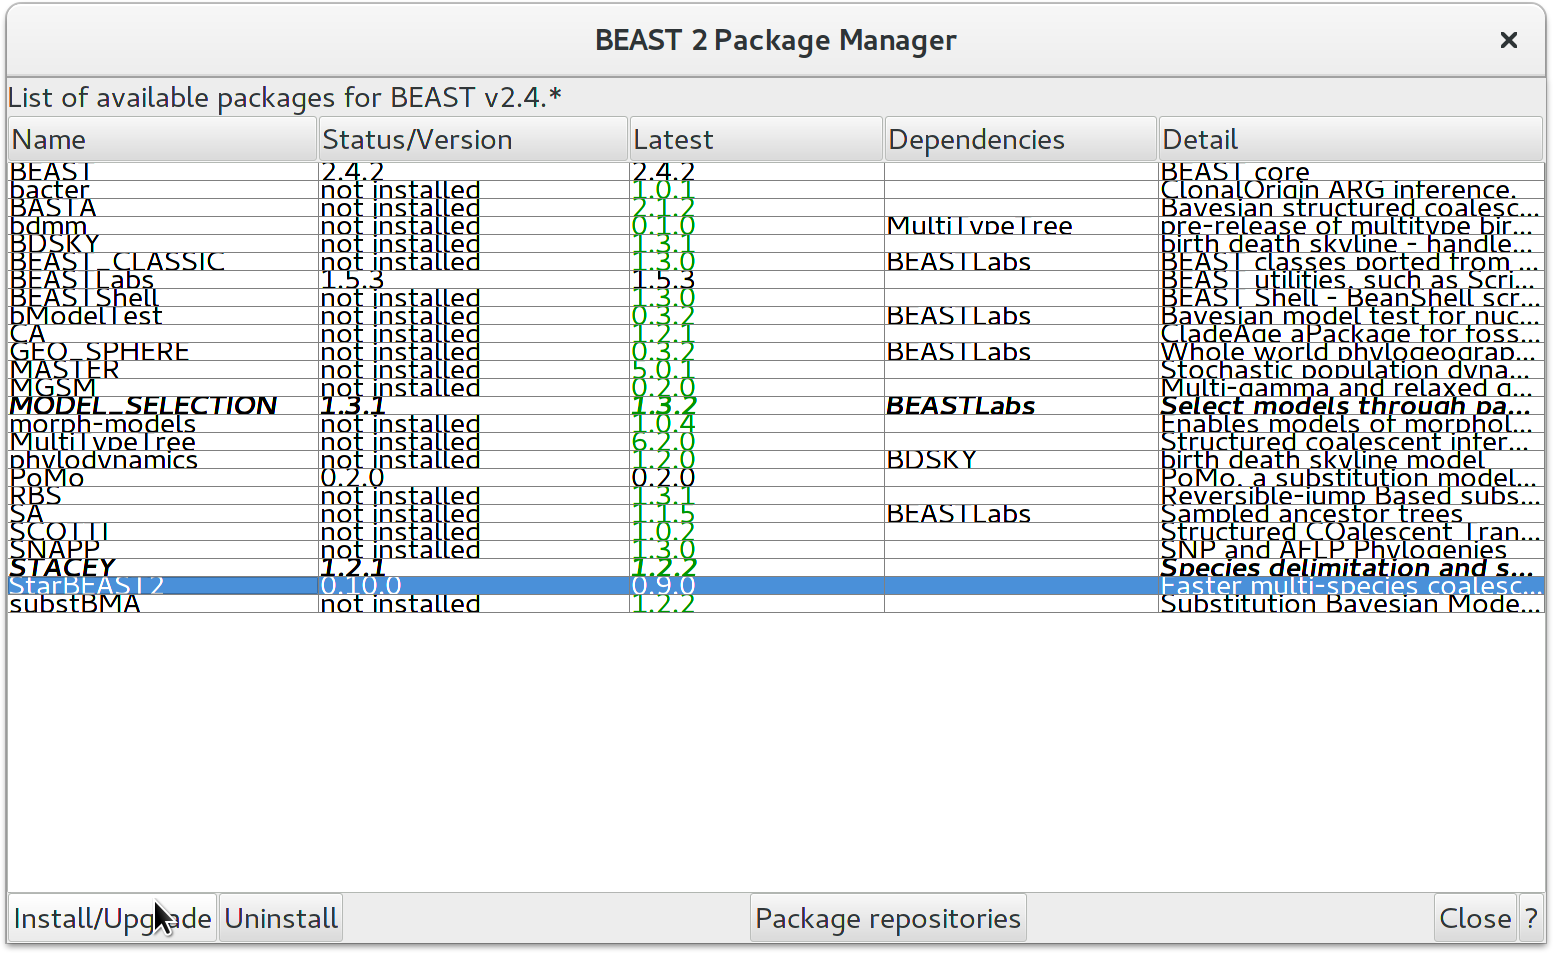
\includegraphics[width=\textwidth]{figures/beauti-install.png}
\caption{Install StarBEAST2 from within BEAUTi.}
\label{fig:managePackages}
\end{figure}

\clearpage

StarBEAST2 includes a series of templates for multispecies coalescent analyses.
These include the \textbf{StarBeast2} template for strict clock or gene tree
relaxed clock analyses, and various \textbf{SpeciesTree\ldots} templates for species tree
relaxed clock analyses. Currently three types of relaxed clocks are supported by
StarBEAST2; the uncorrelated lognormal clock (UCLN), the uncorrelated
exponential clock (UCED), and the random local clock (RLC) which we will use for
this tutorial.  The first thing to do is selecting that template by choosing the
\textbf{File/Template/SpeciesTreeRLC} menu item (Figure~\ref{fig:sb2Template}).
When changing a template, BEAUti deletes all previously imported data and starts
with a new empty template. So, if you already loaded some data, a warning
message pops up indicating that this data will be lost if you switch templates.

\begin{figure}[htb!]
\centering
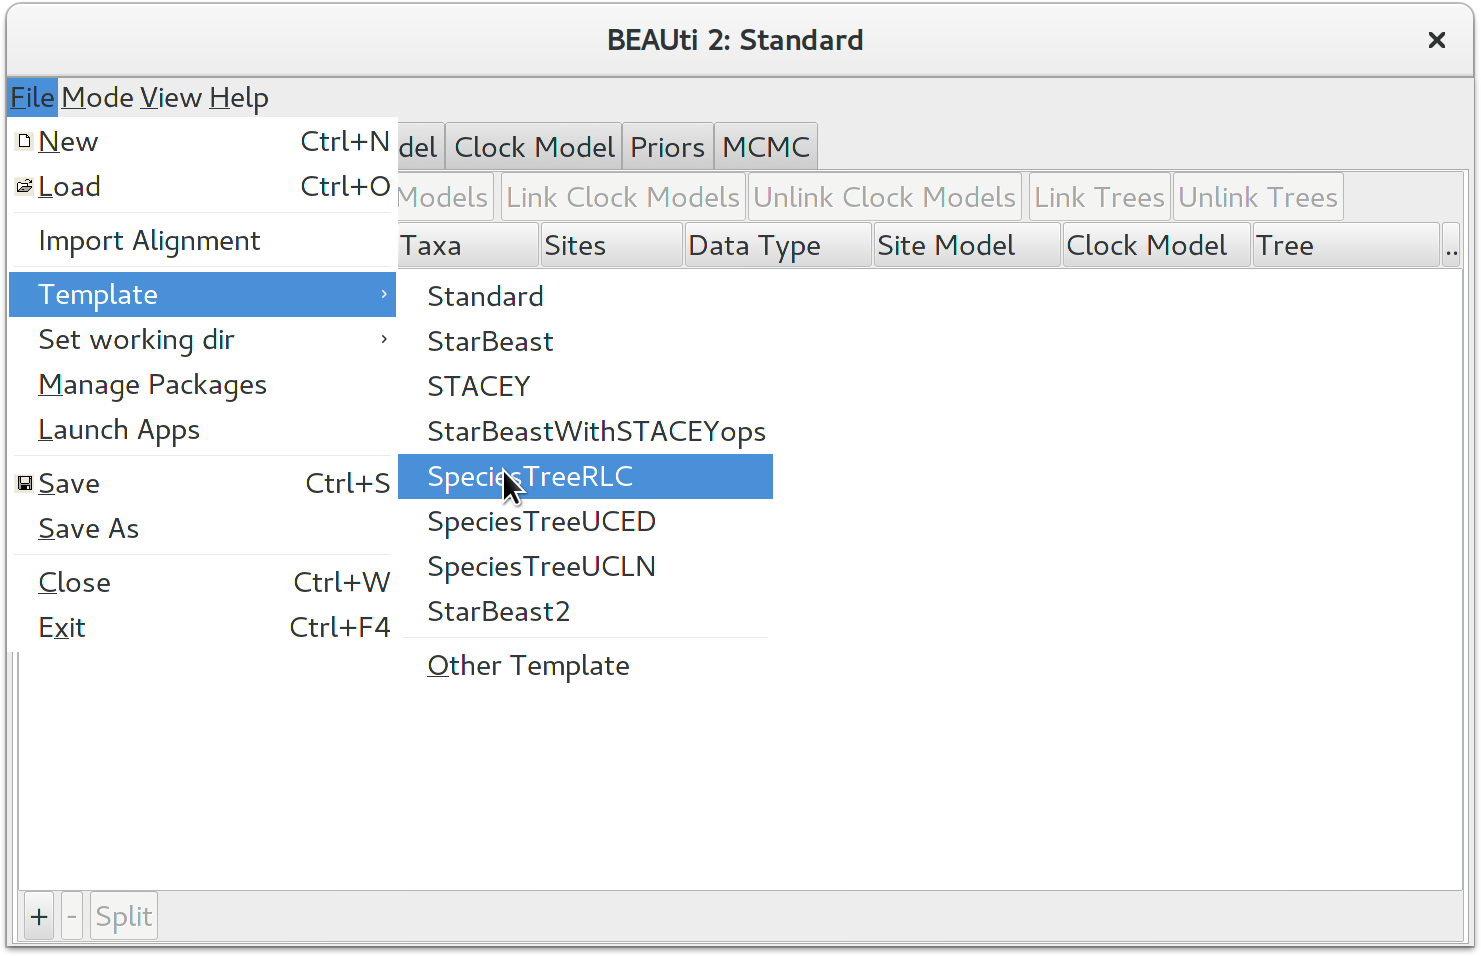
\includegraphics[width=\textwidth]{figures/beauti-rlc.png}
\caption{Select a species tree template in BEAUti.}
\label{fig:sb2Template}
\end{figure}

\clearpage

\subsubsection*{Loading the NEXUS files}

StarBEAST2 supports multiple individuals per-species and multiple loci (we use
the term locus to refer to a genomic sequence, and gene when referring to the
evolutionary tree for a given locus). The data for each locus is stored as one
alignment in its own NEXUS file. Taxa names in each alignment have to be unique,
but duplicates across alignments are fine.

To load a NEXUS format alignment, click the button with the plus symbol ($+$) in
the lower left corner of the main \textbf{Partitions} tab. For this tutorial,
navigate to the \textbf{examples/nexus} subfolder inside the \textbf{beast}
application folder, and select all of the first seven NEXUS files. They should
be numbered 26, 29, 47, 53, 59, 64, and 72 (Figure~\ref{fig:importAlignments}).

\begin{figure}[htb!]
\centering
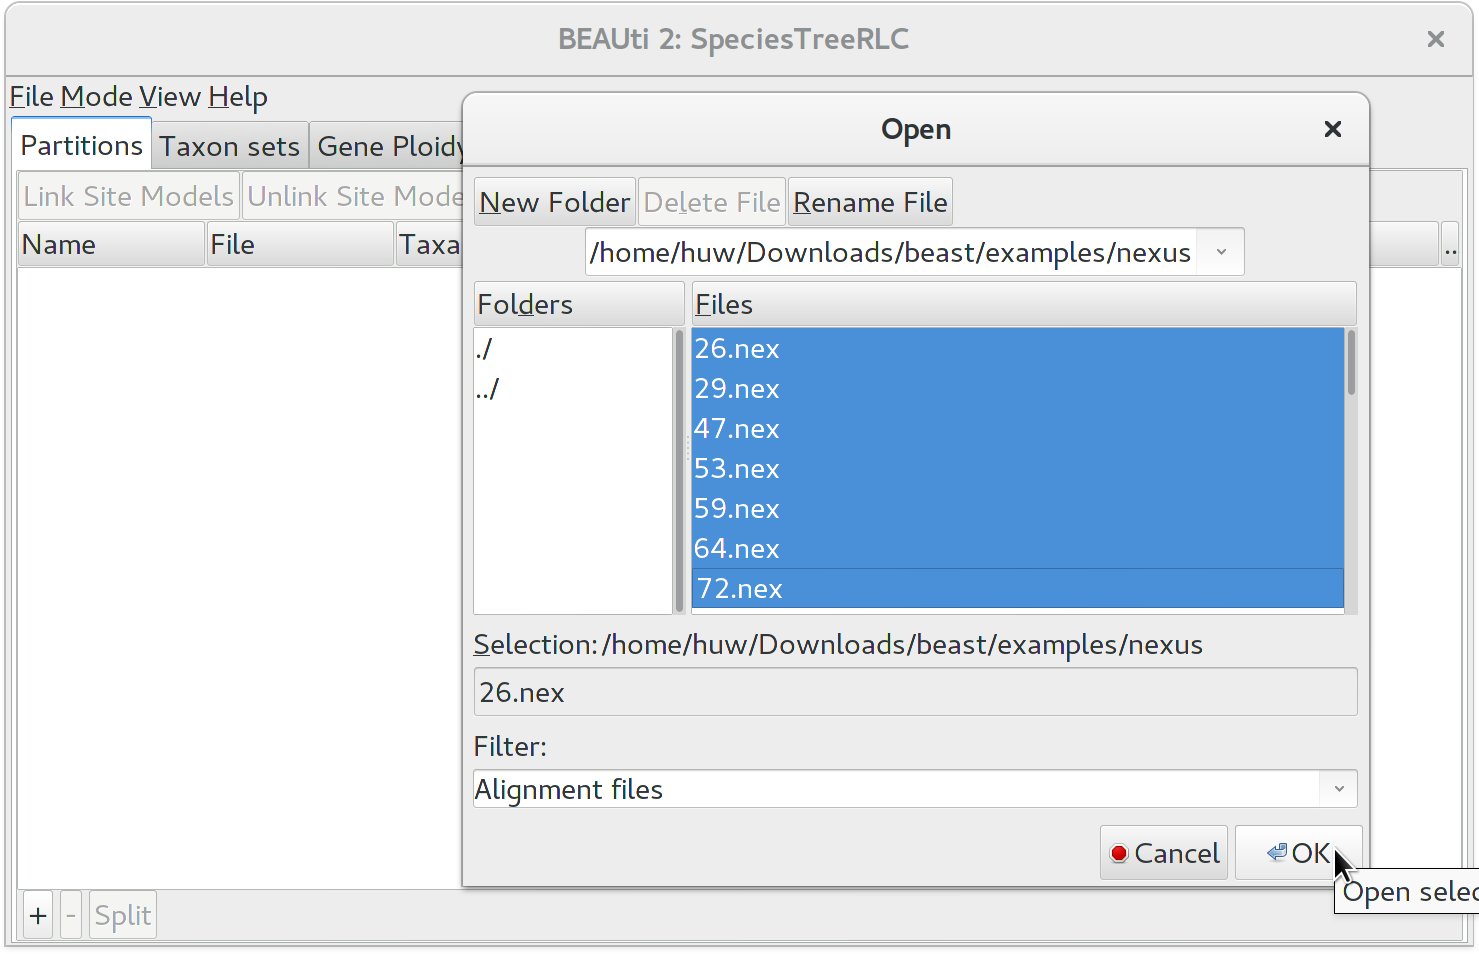
\includegraphics[width=\textwidth]{figures/beauti-import.png}
\caption{Selecting NEXUS alignment files to import.}
\label{fig:importAlignments}
\end{figure}

\clearpage

Each file contains an alignment of sequences of from an independent locus. The
file \textbf{26.nex} looks like this (sequences have been truncated):

\begin{minipage}[h]{0.7\textwidth}
\begin{verbatim}
#NEXUS
[TBO26oLong]
BEGIN DATA;
	DIMENSIONS  NTAX =26 NCHAR=614;
	FORMAT DATATYPE = DNA GAP = - MISSING = ?;
	MATRIX	
  Orthogeomys_heterodus       ATTCTAGGCAAAAAG-AGCAATGC...
  Thomomys_bottae_awahnee_a   ????????????????????ATGC...
  Thomomys_bottae_awahnee_b   ????????????????????ATGC...
  Thomomys_bottae_xerophilus  ????????????????????ATGC...
...

;
END;
\end{verbatim}
\end{minipage}

\vspace{12pt}

Once loaded, the imported alignments are displayed in the \textbf{Partitions}
panel. You can double click any alignment (partition) to show its detail. For
multi-locus analyses, BEAST can link or unlink substitutions models across the
loci by clicking buttons on the top of the panel. The default of StarBEAST2 is
to unlink all models: substitution, clock, and trees. Note
that you should only unlink the tree model across data partitions that are
actually genetically unlinked. For example, in most organisms all the
mitochondrial genes are effectively linked due to a lack of recombination and
they should be set up to use the same tree model in any multispecies coalescent
analysis.

\clearpage

\subsubsection*{Assigning the correct species to each sequence}

%%JH
Each taxon in a StarBEAST2 analysis is associated with a species or similar OTU.
Typically the species name is already embedded inside the taxon label. The
species name should be easy to extract; place it either at the beginning or the
end, separated by a ``special'' character which does not appear in names. For
example, \texttt{aria\_334259, coast\_343436} (using an underscore) or
\texttt{10x017b.wrussia, 2x305b.eastis} (using a dot).
%%JH

We need to tell BEAUti somehow which lineages in the alignments go with taxa in
the species tree. Select the Taxon Set panel, and a list of taxa from the
alignments is shown together with a default guess by BEAUti. In this case, the
guess is not very good, so we want to change this. You can manually change each
of the entries in the table, or press the guess button and a dialog is shown
where you can choose from several ways to try to detect the taxon from the name
of the lineages, or have a mapping stored in a file. In this case, splitting the
name on the underscore character `\_' and selecting the second group will give
us the mapping that we need (Figure~\ref{fig:taxonSets}).

\begin{figure}[htb!]
\centering
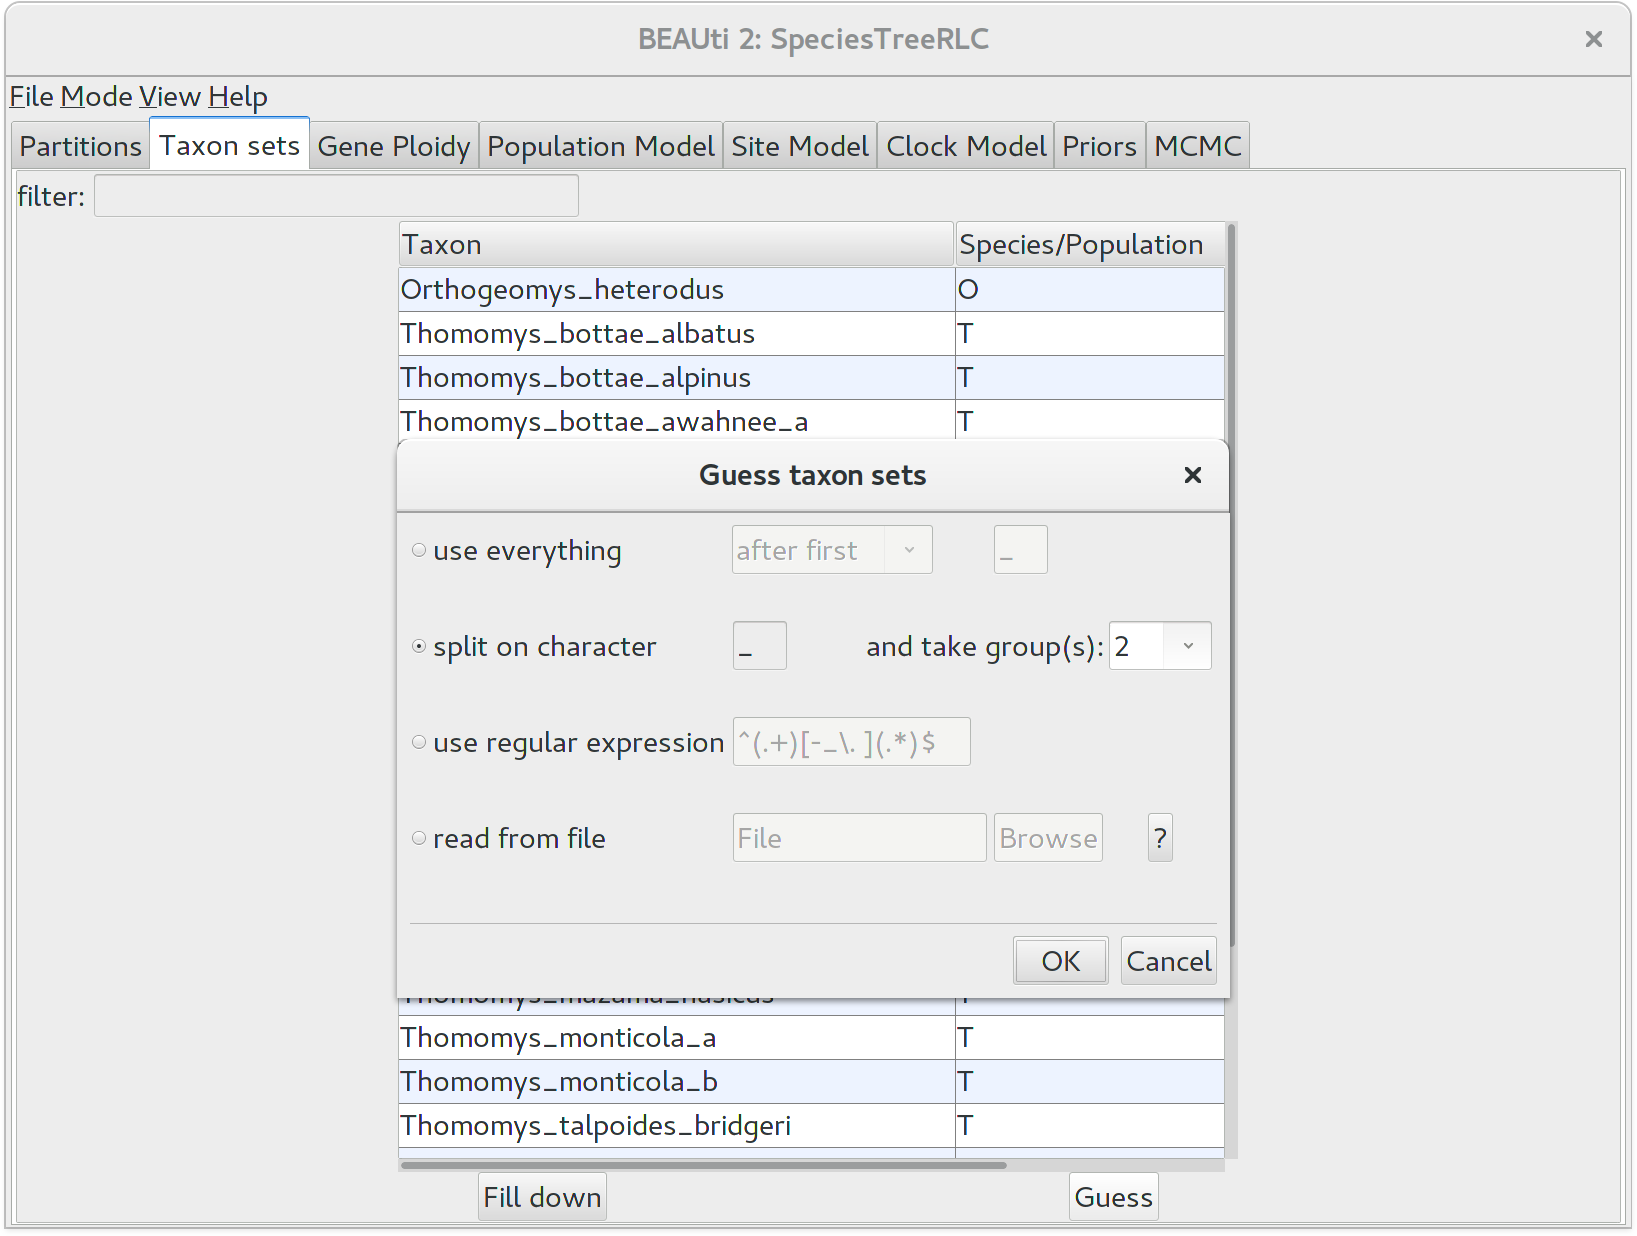
\includegraphics[width=\textwidth]{figures/beauti-guess.png}
\caption{Assigning species to sequences in BEAUti using the guess dialog.}
\label{fig:taxonSets}
\end{figure}

Alternatively, the mapping can be read from a trait file. A proper trait file is
tab delimited. The first row is always \texttt{traits} followed by the keyword
\texttt{species} in the second column and separated by tab. The rest of the rows
map each individual taxon name to a species name: the taxon name in the first
column and species name in the second column separated by tab. For example:

\begin{minipage}[h]{0.7\textwidth}
\begin{verbatim}
traits	species
taxon1	speciesA
taxon2	speciesA
taxon3	speciesB
...
\end{verbatim}
\end{minipage}

\vspace{12pt}

\subsubsection*{Adjusting the ploidy of each gene}

Ploidy should be based on the mode of inheritance for each gene. By convention,
nuclear genes in diploids are given a ploidy of 2.0. Because mitochondrial and Y
chromosome genes are haploid even in otherwise diploid organisms, and also
inherited only through the mother or the father respectively, their effective
population size $N_e$ is only one quarter that of nuclear genes. Therefore if
nuclear gene ploidy is set to 2.0, mitochondrial or Y chromosome gene ploidy
should be set to 0.5. In this analysis all genes are from nuclear loci and their
ploidy should be left at the default value of 2.0.

\clearpage

\subsubsection*{Selecting the method of population size integration}

StarBEAST2, like $\Conv$BEAST before it, can estimate the effective population
sizes for extant and ancestral species. However by default StarBEAST2
analytically integrates over population sizes which is faster than making
explicit estimates. If you do need to estimate population sizes, change the
population model to \textbf{Constant Populations}. For this tutorial, keep the
default model which is \textbf{Analytical Population Size Integration}. In order to improve
convergence of the MCMC chain, set the population size mean to 0.003 and uncheck
the option to estimate this value (Figure~\ref{fig:pop}). \textcolor{red}{For
real analyses you should almost certainly estimate this value, but a fixed value
will help us complete the tutorial in a reasonable time frame.}

\begin{figure}[htb!]
\centering
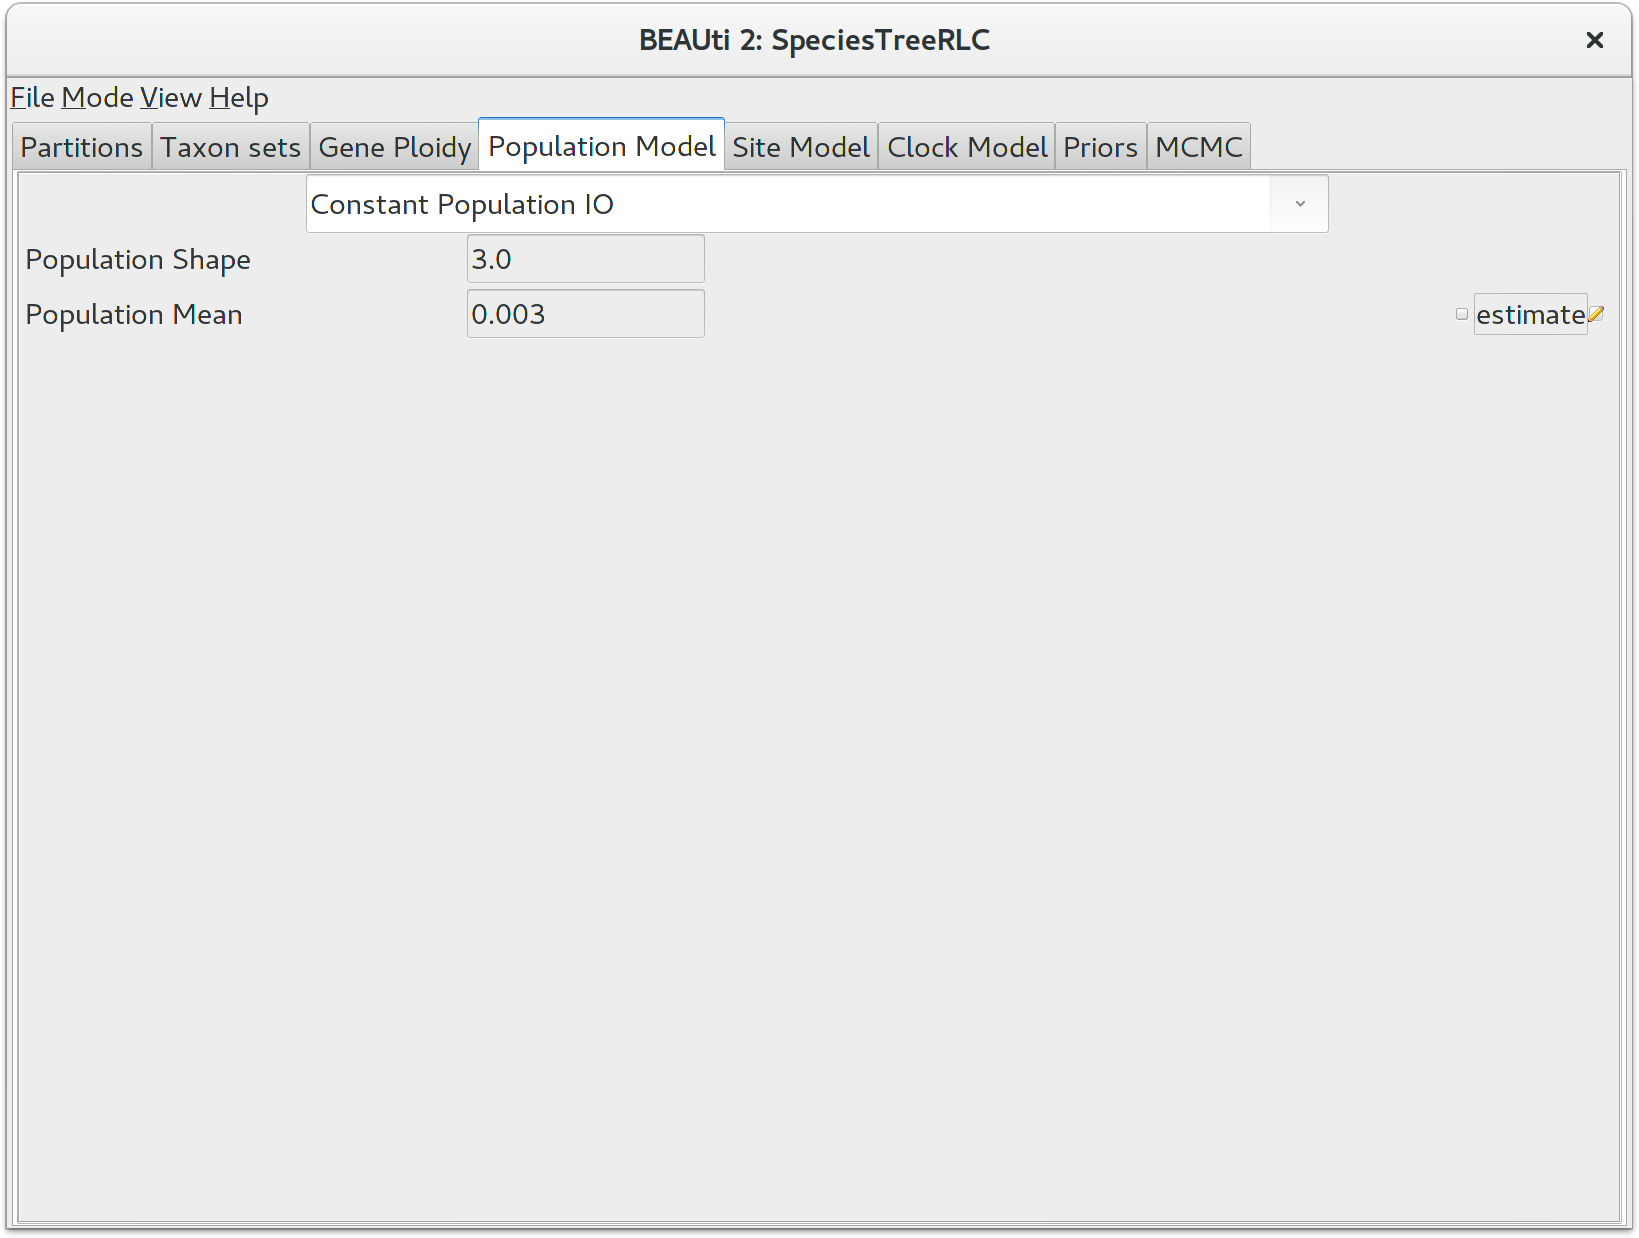
\includegraphics[width=\textwidth]{figures/beauti-pop-model.png}
\caption{The choice of population models used by StarBEAST2.}
\label{fig:pop}
\end{figure}

\clearpage

\subsubsection*{Setting the substitution model}

The next thing to do is to click on the \textbf{Site Model} tab at the top of
the main window. This will reveal the evolutionary model settings for BEAST.
Exactly which options appear depend on whether the data are nucleotides, or
amino acids, or binary data, or general data. The settings that will appear
after loading the data set will be the default values so we need to make some
changes.

Many of the models may be familiar to you. For this analysis, we will select
each substitution model listed on the left side in turn to make the following
change: select ``HKY'' for substitution model (\textbf{Subst Model} in
Figure~\ref{fig:HKY}). Make sure to repeat this step for every partition listed
on the left side.

\begin{figure}[htb!]
\centering
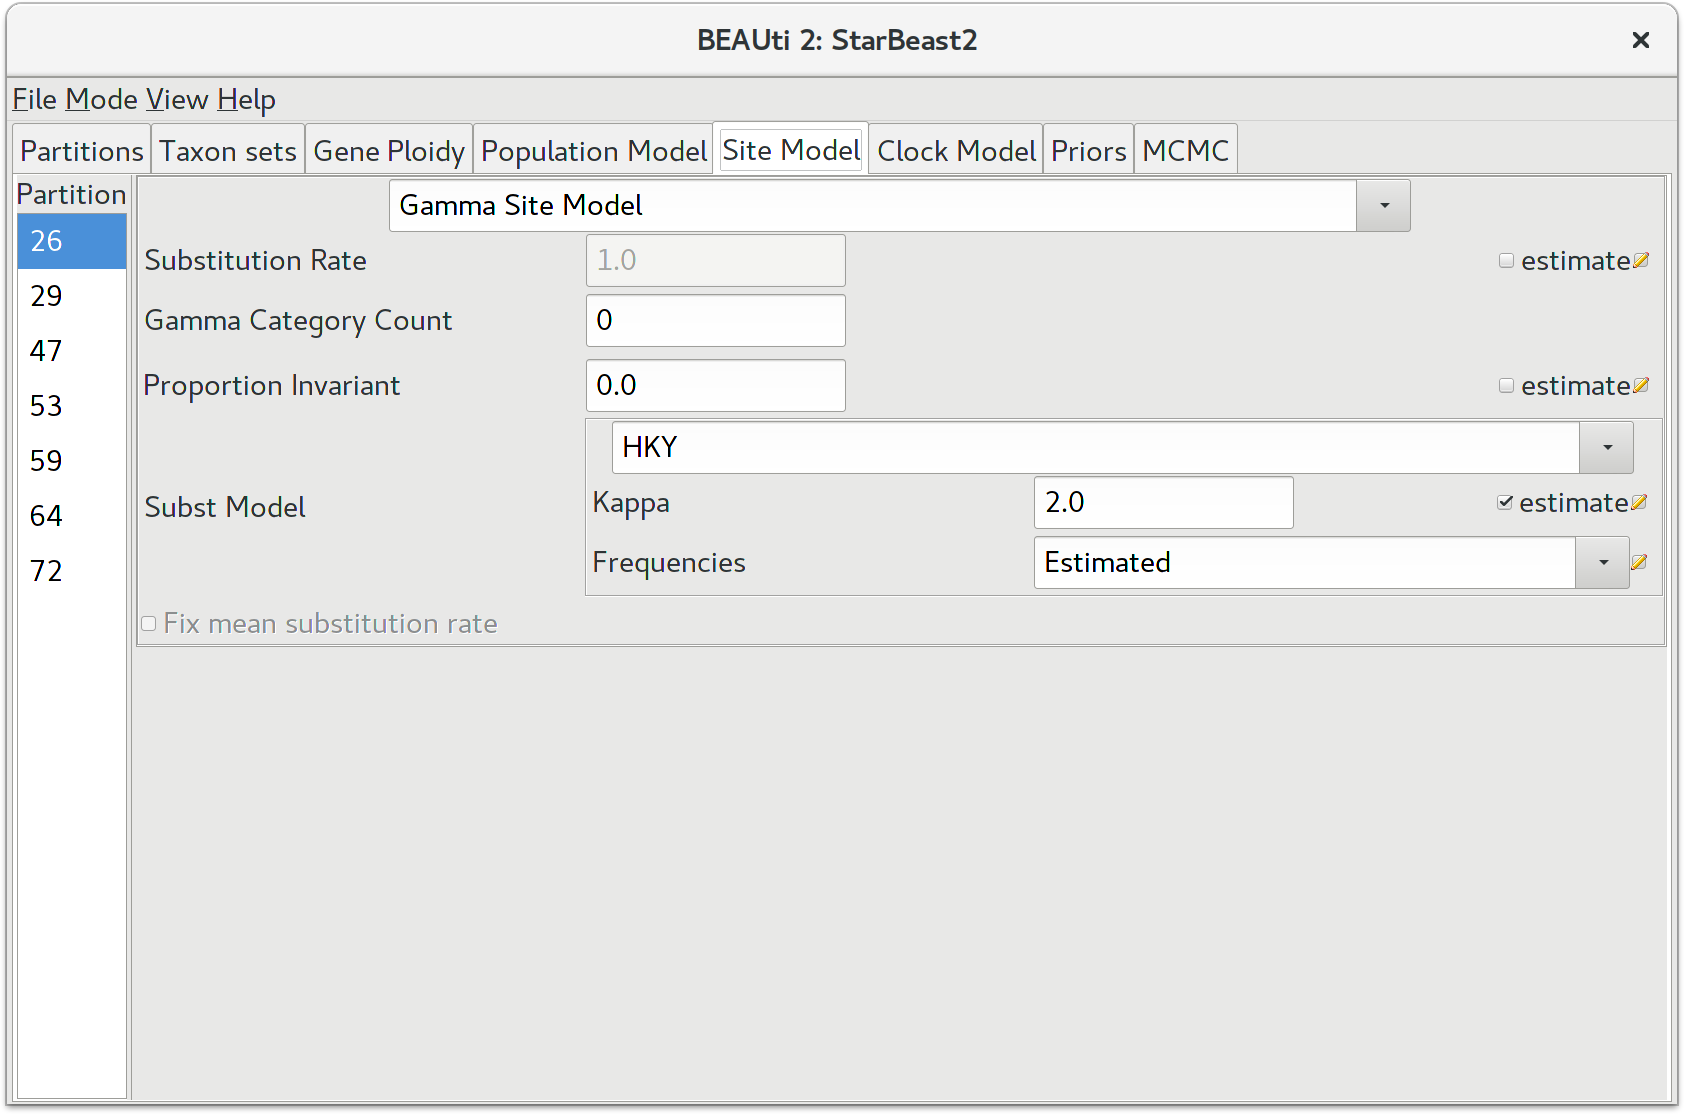
\includegraphics[width=\textwidth]{figures/beauti-hky.png}
\caption{Setting up substitution and site models for the gopher alignments.}
\label{fig:HKY}
\end{figure}

\clearpage

\subsubsection*{Setting the clock model}

Click on the \textbf{Clock Model} tab at the top of the main window. In this
panel you can configure the mean clock rate for each locus. The
mean clock rate ``Clock.rate'' of all partitions should have the
\textbf{estimate} box ticked (Figure~\ref{fig:clock}).

\begin{figure}[htb!]
\centering
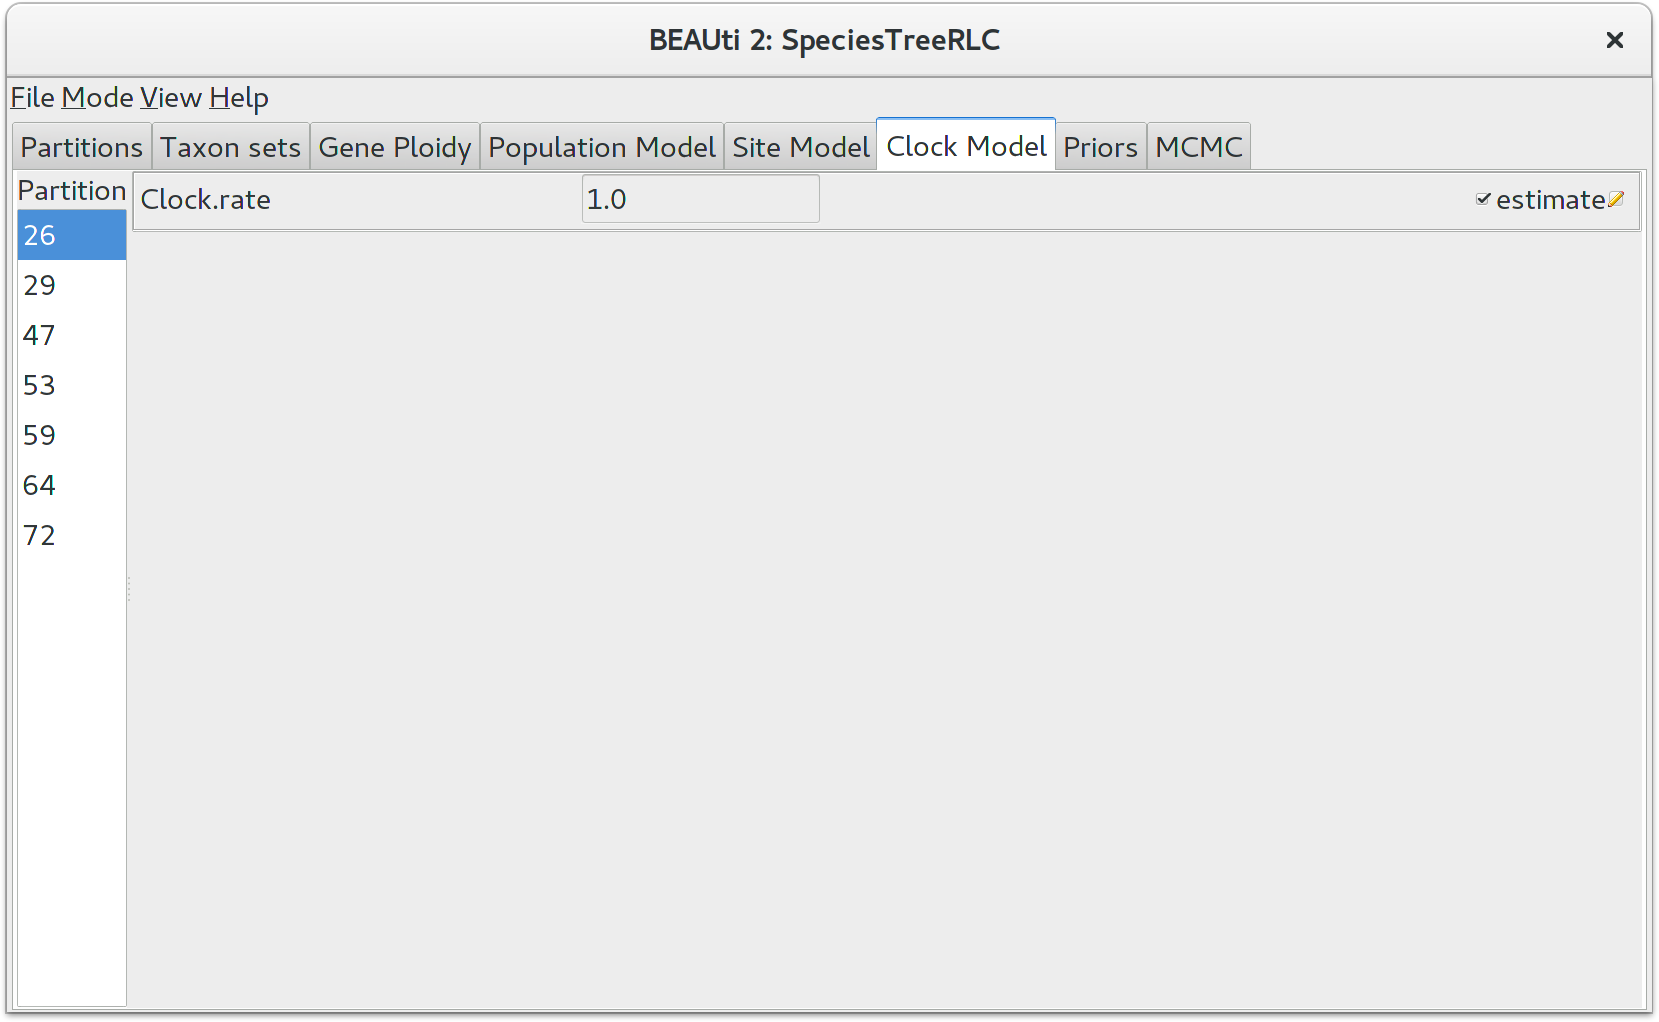
\includegraphics[width=\textwidth]{figures/beauti-clock.png}
\caption{The default when automatic clock rate setting is disabled.}
\label{fig:clock}
\end{figure}

The default prior for mean clock rates in StarBEAST2 is a lognormal distribution
with a mean (in real space) of 1. Trees estimated using this prior will have a
time axis in units of substitutions. This will not be appropriate when using
fossil (or other external) calibrations. You might instead use a 1/X prior,
which is uninformative and will allow the calibration(s) to guide the clock
rates.

\clearpage

\subsubsection*{Priors}

The \textbf{Priors} panel allows priors to be specified for each parameter in
the model. Click the top-leftmost arrow to expand the options available for the
default ``Yule Model'', and set the speciation rate (called for some silly
historical reason ``Birth Diff Rate'') to 180.0. Uncheck the
\textbf{estimate} box to make this a fixed parameter (Figure~\ref{fig:yule}). \textcolor{red}{For real
analyses you should almost certainly estimate this value, but a fixed value will
help us complete the tutorial in a reasonable time frame.}

\begin{figure}[htb!]
\centering
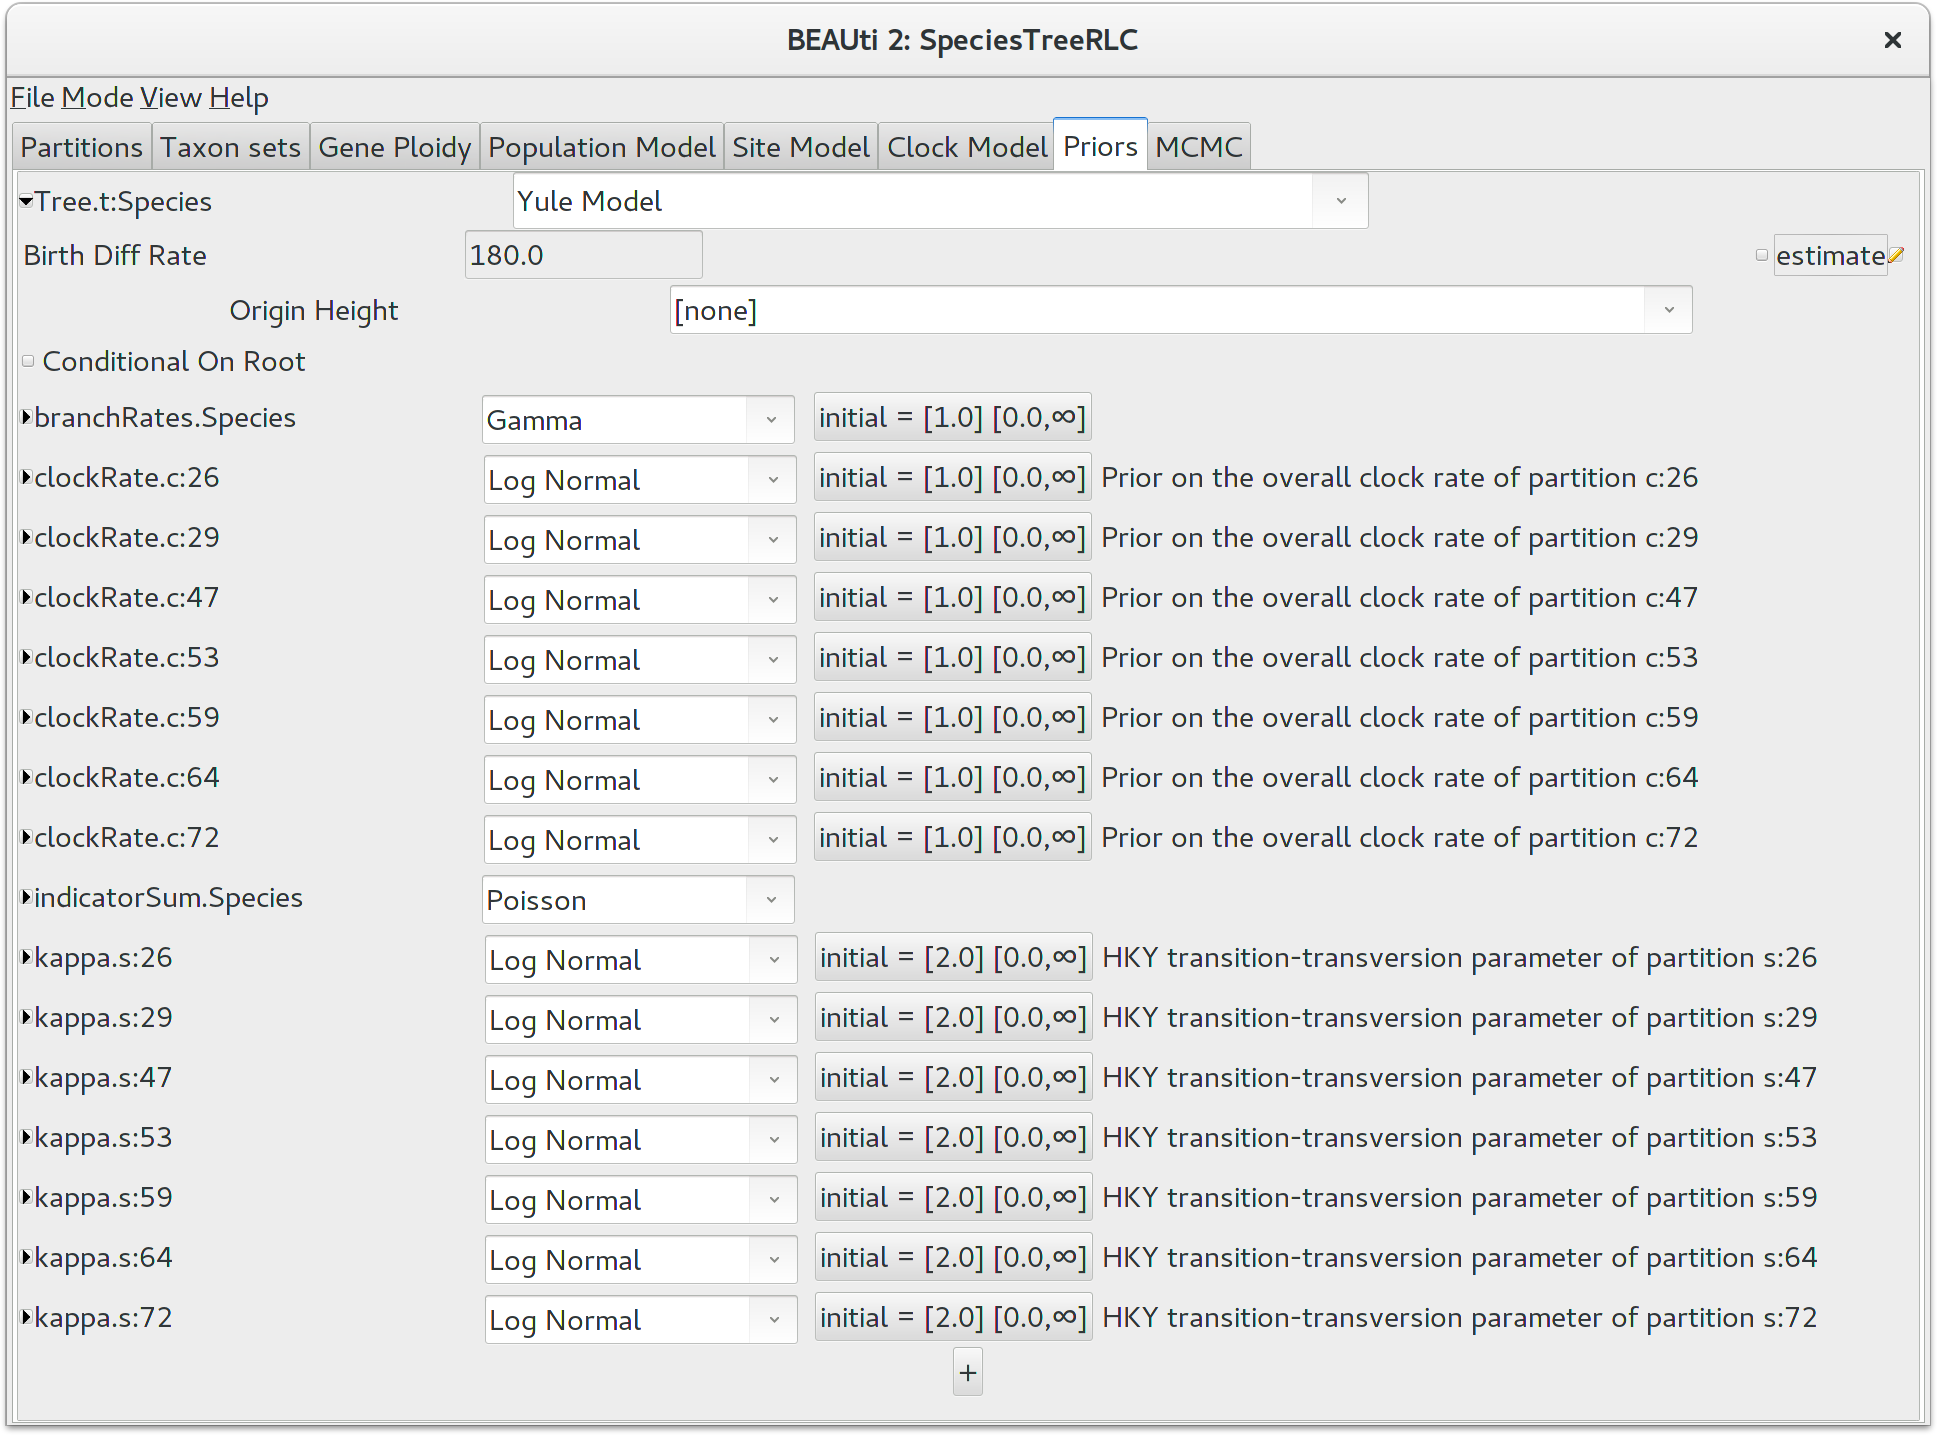
\includegraphics[width=\textwidth]{figures/beauti-yule.png}
\caption{Fixing the speciation rate.}
\label{fig:yule}
\end{figure}

It would be biologically implausible for closely related species to have very large
differences in substitution rates, so we should constrain the per-species branch
rates to a reasonable range of values. Click the button next to
``branchRates.Species'' to define this range. Change ``Lower'' to 0.1 and
``Upper'' to 10.0, which means that the fastest branch rate can not be more than
$100\times$ that of the slowest branch rate (Figure~\ref{fig:limits}).

\begin{figure}[htb!]
\centering
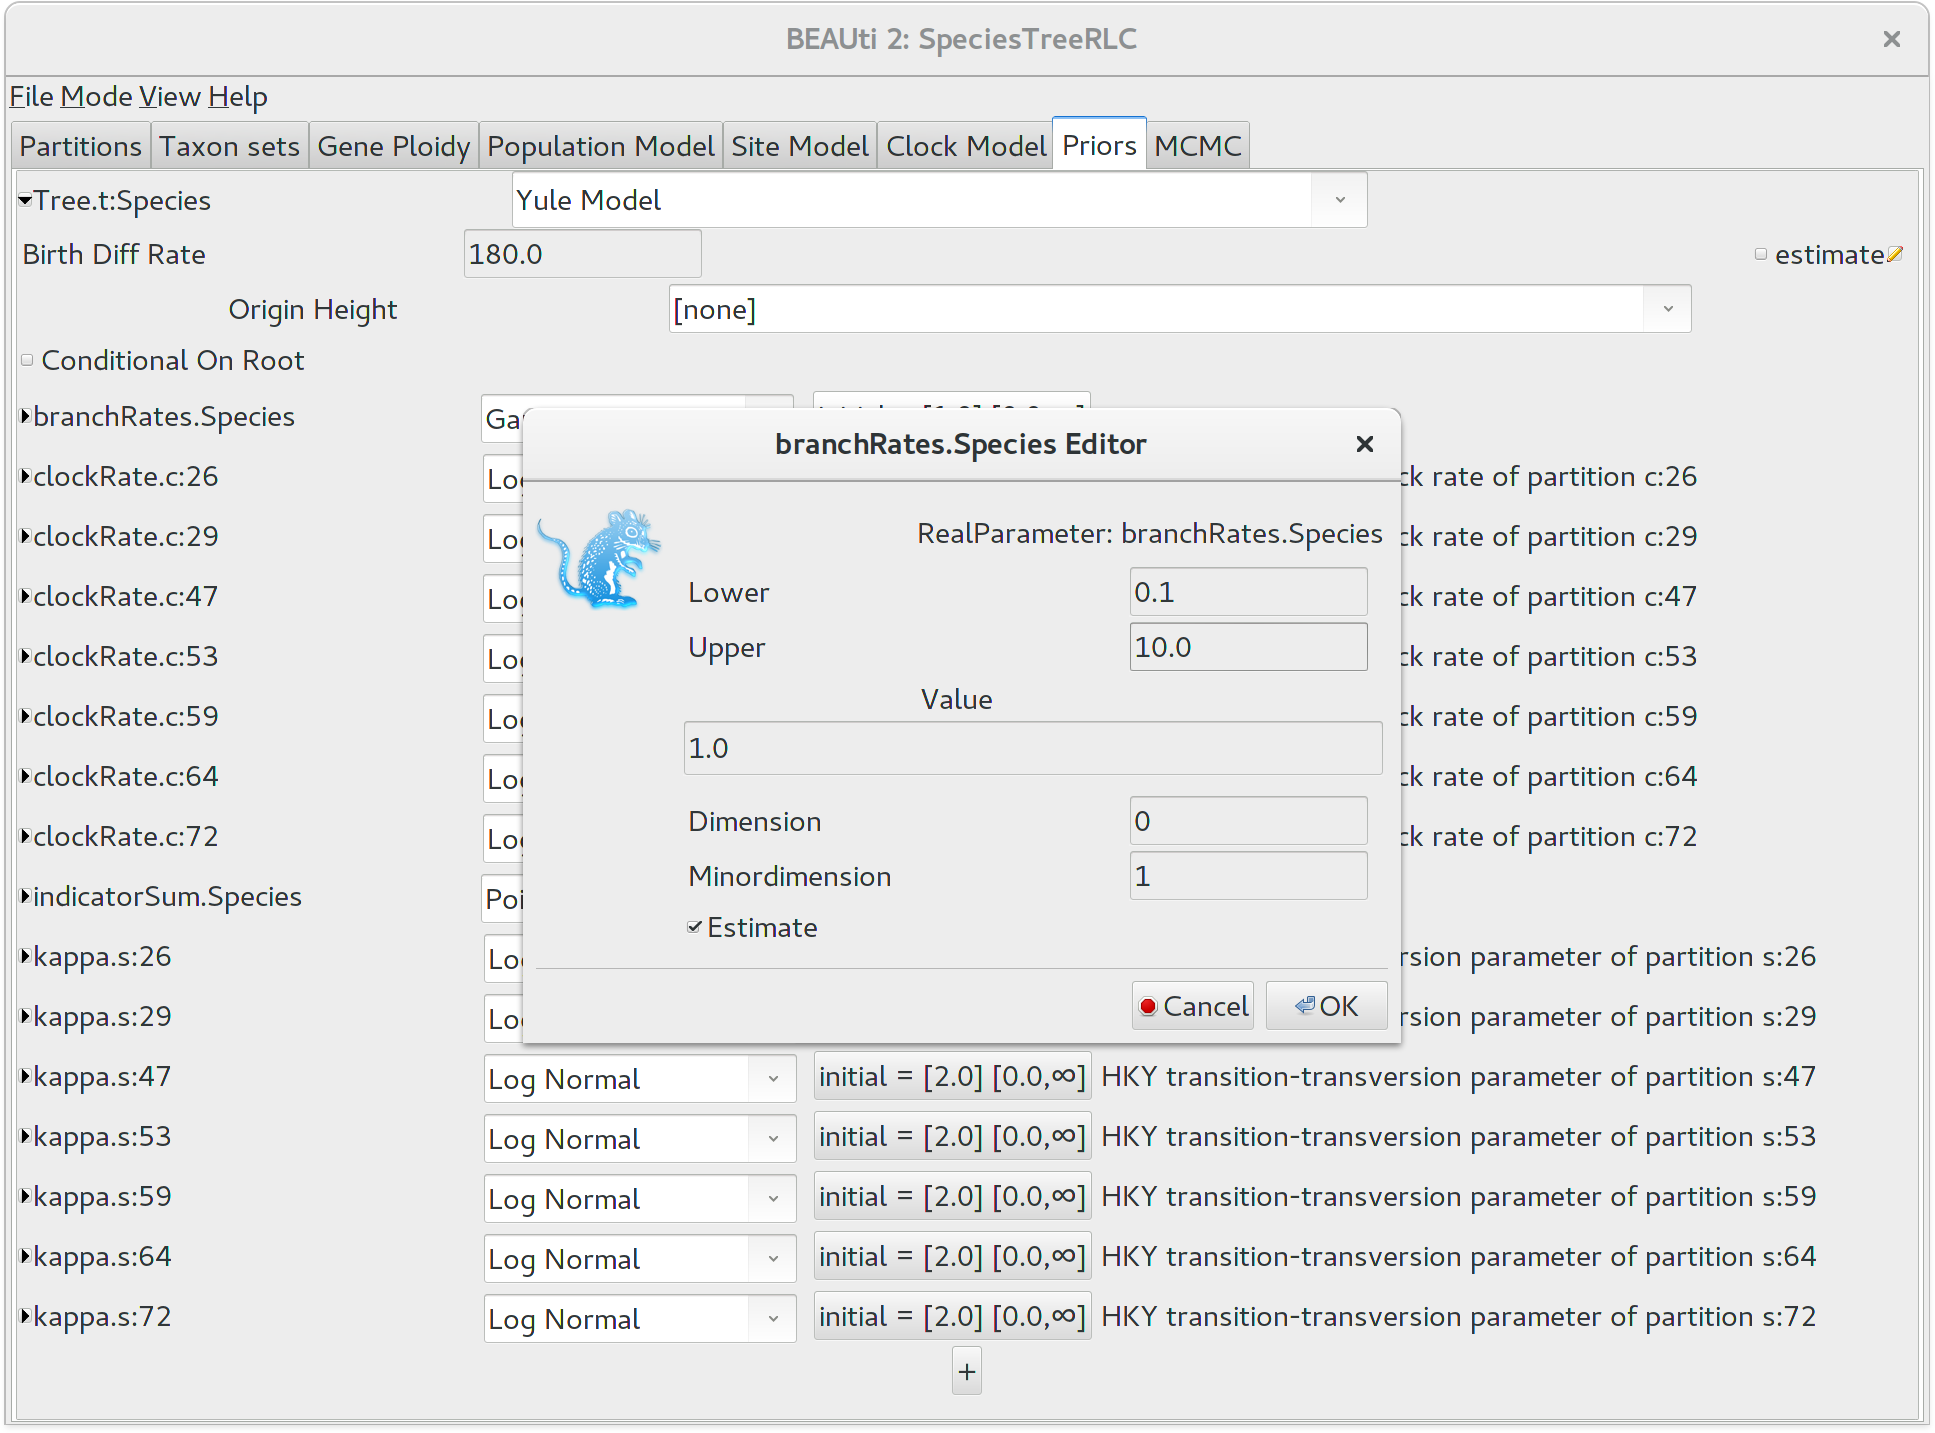
\includegraphics[width=\textwidth]{figures/beauti-branch-rates.png}
\caption{Setting reasonable limits on species branch rates.}
\label{fig:limits}
\end{figure}

\subsubsection*{Setting the MCMC options }

The next tab, \textbf{MCMC}, provides more general settings to control the
length of the MCMC and the file names.

First up is the \textbf{Chain Length}. This the number of steps BEAST will
complete before stopping an MCMC chain. The appropriate length of the chain
depends on the size of the data set, the complexity of the model and on the
accuracy of the answer required. The default value of 10,000,000 is entirely
arbitrary and should be adjusted according to the size of your data set. For
this tutorial keep the default chain length, which should finish within 20
to 30 minutes on a modern computer (Figure~\ref{fig:mcmc}).

\begin{figure}[htb!]
\centering
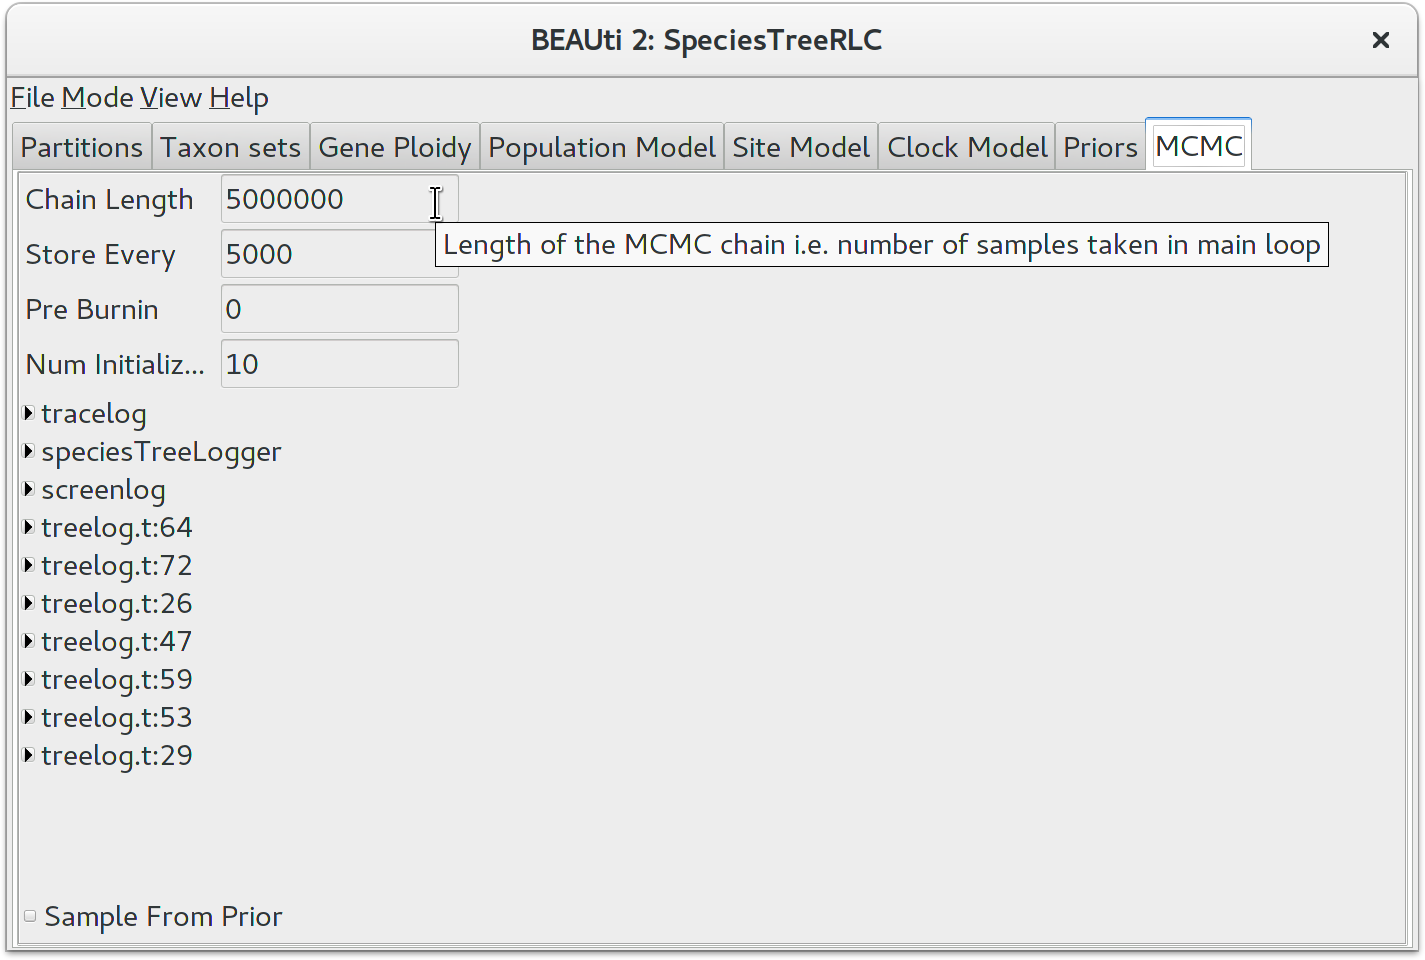
\includegraphics[width=\textwidth]{figures/beauti-mcmc.png}
\caption{Setting up the MCMC paremeters.}
\label{fig:mcmc}
\end{figure}

The other options specify how the parameter values in the Markov chain should be
displayed on the screen and recorded in the log file. The \textbf{screenlog} output is
simply for monitoring the programs progress so can be set to any value (although
if set too small, the sheer quantity of information being displayed on the
screen will actually slow the program down). For the \textbf{tracelog} and \textbf{treelog} files, the value should
be set relative to the total length of the chain. Sampling too often will result
in very large files with little extra benefit in terms of the precision of the
analysis. Sample too infrequently and the log file will not contain much
information about the distributions of the parameters. You probably want to aim
to store no more than $10000$ samples so this should be set to no less than
$\text{chain length}\div10000$. For this exercise, leave the default \textbf{Store
Every} and \textbf{Log Every} settings in place.

If you are using Windows then we suggest you add the suffix ``.txt'' to the
tracelog, speciesTreeLog, and other treelog file names (e.g.
``starbeast.log.txt'' and ``species.trees.txt'') so that Windows recognizes them as text files.

\subsubsection*{Generating the BEAST XML file}

We are now ready to create the BEAST XML file. To do this, either select the
\textbf{File/Save} or \textbf{File/Save~As} menu options. Save the file with an
appropriate name (we usually end the filename with ``.xml'', e.g.
``pocket-gophers-rlc.xml''). We are now ready to run the file through BEAST.

\subsection*{Running BEAST}

Now run BEAST and when it asks for an input file, provide your newly created XML
file as input by clicking \textbf{Choose~File...}, and then click \textbf{Run}.
In Linux BEAST will immediately launch a file opening dialog box, which is to
select the BEAST XML to run. BEAST will then run until it has finished reporting
information to the screen. The actual results files are saved to the disk in the
same location as your input file. The output to the screen will look something
like this:

{\scriptsize
\begin{verbatim}
                   BEAST v2.4.3 Prerelease, 2002-2016
             Bayesian Evolutionary Analysis Sampling Trees
                       Designed and developed by
 Remco Bouckaert, Alexei J. Drummond, Andrew Rambaut & Marc A. Suchard
...

         Sample      posterior ESS(posterior)     likelihood          prior
              0     -9462.6137              N    -10189.1746       -49.6988 --
           5000     -9385.6106         2.0       -10010.6403       -26.3203 --
...

        9995000     -9101.9036       998.4        -9807.8587       -20.1634 1m57s/Msamples
       10000000     -9120.5011       999.6        -9820.1012       -23.5461 1m57s/Msamples

Operator                                                                Tuning    #accept    #reject      Pr(m)  Pr(acc|m)
ScaleOperator(branchRateScaler.Species)                                 0.1764      44970     119601     0.0164     0.2733 
BitFlipOperator(indicatorFlipper.Species)                                    -       3242      78885     0.0082     0.0395 
NodeReheight(Reheight.t:Species)                                             -      88386     596000     0.0685     0.1291 
starbeast2.CoordinatedUniform(coordinatedUniform.t:Species)                  -      49238      87613     0.0137     0.3598 
starbeast2.CoordinatedExponential(coordinatedExponential.t:Species)     0.0024      46894      90442     0.0137     0.3415 
ScaleOperator(TreeScaler.t:Species)                                     0.9717       5829      21463     0.0027     0.2136 
ScaleOperator(TreeRootScaler.t:Species)                                 0.6680       5341      21908     0.0027     0.1960 
Uniform(UniformOperator.t:Species)                                           -      15811     121214     0.0137     0.1154 
SubtreeSlide(SubtreeSlide.t:Species)                                    0.0012      24270     111965     0.0137     0.1781 
Exchange(Narrow.t:Species)                                                   -      13725     123242     0.0137     0.1002 
Exchange(Wide.t:Species)                                                     -       1620     135249     0.0137     0.0118 
WilsonBalding(WilsonBalding.t:Species)                                       -        455     136871     0.0137     0.0033 
UpDownOperator(updown.all.Species)                                      0.4177      14847      39909     0.0055     0.2711 
ScaleOperator(clockRateScaler.c:64)                                     0.5266       8901      29944     0.0038     0.2291 
UpDownOperator(clockUpDownOperator.c:64)                                0.9097      10820      27497     0.0038     0.2824 
ScaleOperator(TreeScaler.t:64)                                          0.9146      10571      27821     0.0038     0.2753 
ScaleOperator(TreeRootScaler.t:64)                                      0.4977       7532      30987     0.0038     0.1955 
Uniform(UniformOperator.t:64)                                                -      93357      97911     0.0192     0.4881 
SubtreeSlide(SubtreeSlide.t:64)                                         0.0040      31114     160448     0.0192     0.1624 
Exchange(Narrow.t:64)                                                        -      51189     139889     0.0192     0.2679 
Exchange(Wide.t:64)                                                          -       2512     189065     0.0192     0.0131 
WilsonBalding(WilsonBalding.t:64)                                            -       2440     189974     0.0192     0.0127 
...

ScaleOperator(KappaScaler.s:26)                                         0.3459       3993       8772     0.0013     0.3128 
...

DeltaExchangeOperator(FrequenciesExchanger.s:47)                        0.0907       3578      15709     0.0019     0.1855 
...

     Tuning: The value of the operator's tuning parameter, or '-' if the operator can't be optimized.
    #accept: The total number of times a proposal by this operator has been accepted.
    #reject: The total number of times a proposal by this operator has been rejected.
      Pr(m): The probability this operator is chosen in a step of the MCMC (i.e. the normalized weight).
  Pr(acc|m): The acceptance probability (#accept as a fraction of the total proposals for this operator).


Total calculation time: 1180.325 seconds
End likelihood: -9120.501194044526
\end{verbatim}}

\section{Analyzing the results}

Run the program called \textbf{Tracer} to analyze the output of BEAST. When the
main window has opened, choose \textbf{Import Trace File...} from the
\textbf{File} menu and select the file that BEAST has created called
``starbeast.log''. On the left hand side is a list of the different quantities
that BEAST has logged. There are traces for the the various probabilities and
likelihoods as well as estimates of various discrete and continuous parameters.
The first and most important trace --- the ``posterior'' --- is the log of the
product of gene tree phylogenetic likelihoods, the coalescent probability of
gene trees within the species tree, and all prior probabilities.
Selecting a trace on the left brings up analyses for this trace on the right
hand side depending on tab that is selected. Select the statistic named
``sum(indicators.Species)'' --- this is the total number of substitution rate
changes along the species tree. You should now see a window like in Figure
\ref{fig:tracer}.

\begin{figure}[htb!]
\centering
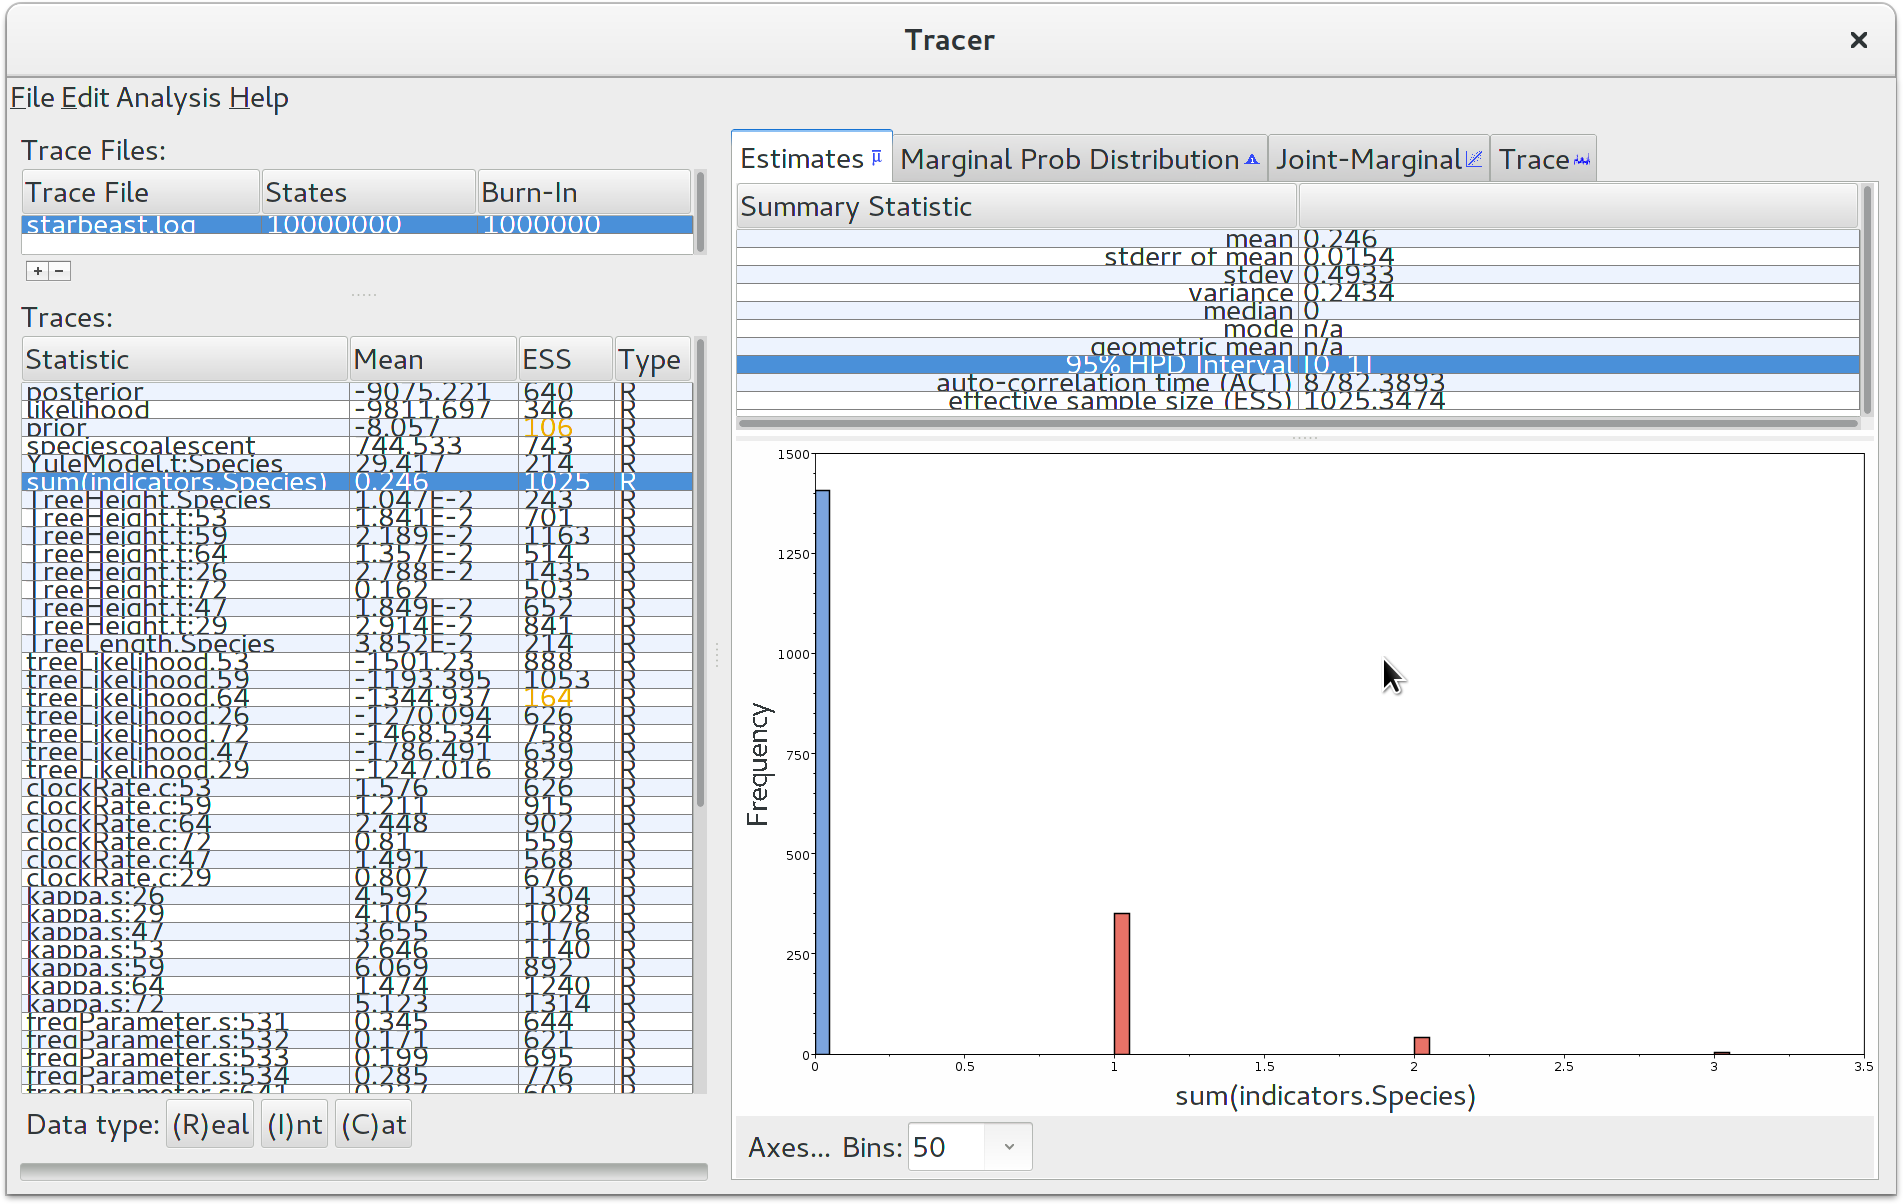
\includegraphics[width=\textwidth]{figures/tracer-posterior.png}
\caption{Tracer with the gopher data.}
\label{fig:tracer}
\end{figure}

Remember that MCMC is a stochastic algorithm so the actual numbers will not be
exactly the same. Tracer will plot a (marginalized) posterior distribution for
the selected parameter and also give you statistics such as the mean and median.
The ``95\% HPD interval'' stands for \textit{highest posterior density
interval}, and represents the most compact interval on the selected parameter
that contains 95\% of the posterior probability. It is also known as a
\textit{credibility interval}, and can be thought of as a Bayesian analog to a
confidence interval. The HPD for the sum of rate changes suggests that either 0,
1 or 2 rate changes have occured.

\subsection*{A note on prior distributions}

For any Bayesian analysis, it is very important to compare your findings with
the prior distribution. The default prior distribution for the number of
substitution rate shifts for a random local clock is a Poisson distribution
with the $\lambda$ parameter fixed at $\ln(2) \approx 0.69$. The prior
probability of zero rate changes for the default distribution is equal to
50\%. Tracer reported that around 1250 samples had zero rate shifts,
out of $9000000 \div 5000 = 1800$ post-burnin posterior samples. This means that after
adding data, our belief in a strict clock increased from 50\% to about 70\%,
a very modest change. The data in this tutorial suggests that a strict clock
applies to pocket gophers, but falls far short of any standard of proof.

\subsection*{Obtaining an estimate of the phylogenetic tree}

BEAST also produces a sample of plausible trees. These can be summarized using
the program \textbf{TreeAnnotator}. This will take the set of trees and identify
a single tree that best represents the posterior distribution. It will then
annotate this selected tree topology with the mean ages of all the nodes as well
as the 95\% HPD interval of divergence times for each clade in the selected
tree. It will also calculate the posterior clade probability for each node. Run
the \textbf{TreeAnnotator} program and set it up to look like in
Figure~\ref{fig:treeannotator}.

\begin{figure}[htb!]
\centering
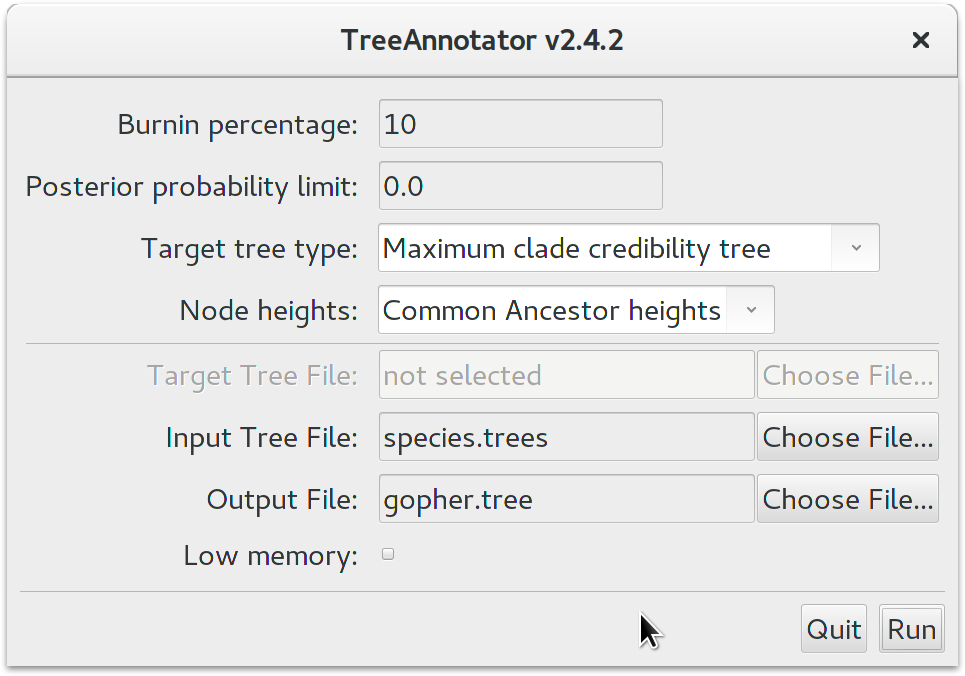
\includegraphics[width=0.7\textwidth]{figures/treeannotator.png}
\caption{Using TreeAnnotator to summarise the tree set.}
\label{fig:treeannotator}
\end{figure}

The \textbf{Burnin percentage} is the proportion of trees to remove from the
start of the sample; for this tutorial, set a 10\% burnin as shown in
Figure~\ref{fig:treeannotator}.

The \textbf{Posterior probability limit} option specifies a limit such that if a
node is found at less than this frequency in the sample of trees (i.e., has a
posterior probability less than this limit), it will not be annotated.

For \textbf{Target tree type} you can either choose a specific tree from a file
or ask TreeAnnotator to find a tree in your sample. The default option,
\textbf{Maximum clade credibility tree}, finds the tree with the highest product
of the posterior probability of all its nodes.

Keep ``Common Ancestor heights'' for \textbf{Node heights}. This sets the
heights (ages) of each node in the tree to the mean height of the most recent
common ancestor across the entire set of trees in the posterior.

For the input file, select the trees file that BEAST created (by default this
will be called ``species.trees'') and select a file for the output (here we
have called it ``pocket-gophers.tree''). Now press \textbf{Run} and wait for the
program to finish.

\subsection*{Viewing the species tree(s)}

Finally, we can look at the tree in another program called \textbf{FigTree}. Run
this program, and open the ``pocket-gophers.tree'' file by using the Open command
in the File menu. The tree should appear. You can now try selecting some of the
options in the control panel on the left. Try selecting \textbf{Node Bars} to
get node age error bars. Turn on \textbf{Node Labels} and select
``posterior'' to get it to display the posterior probability for each node,
and also turn on \textbf{Branch Labels} and select ``rate\_95\%\_HPD'' to display
the 95\% HPD of the relative substitution rate for each species tree branch.
You should end up with something like Figure \ref{fig:figtree}.

\begin{figure}[htb!]
\centering
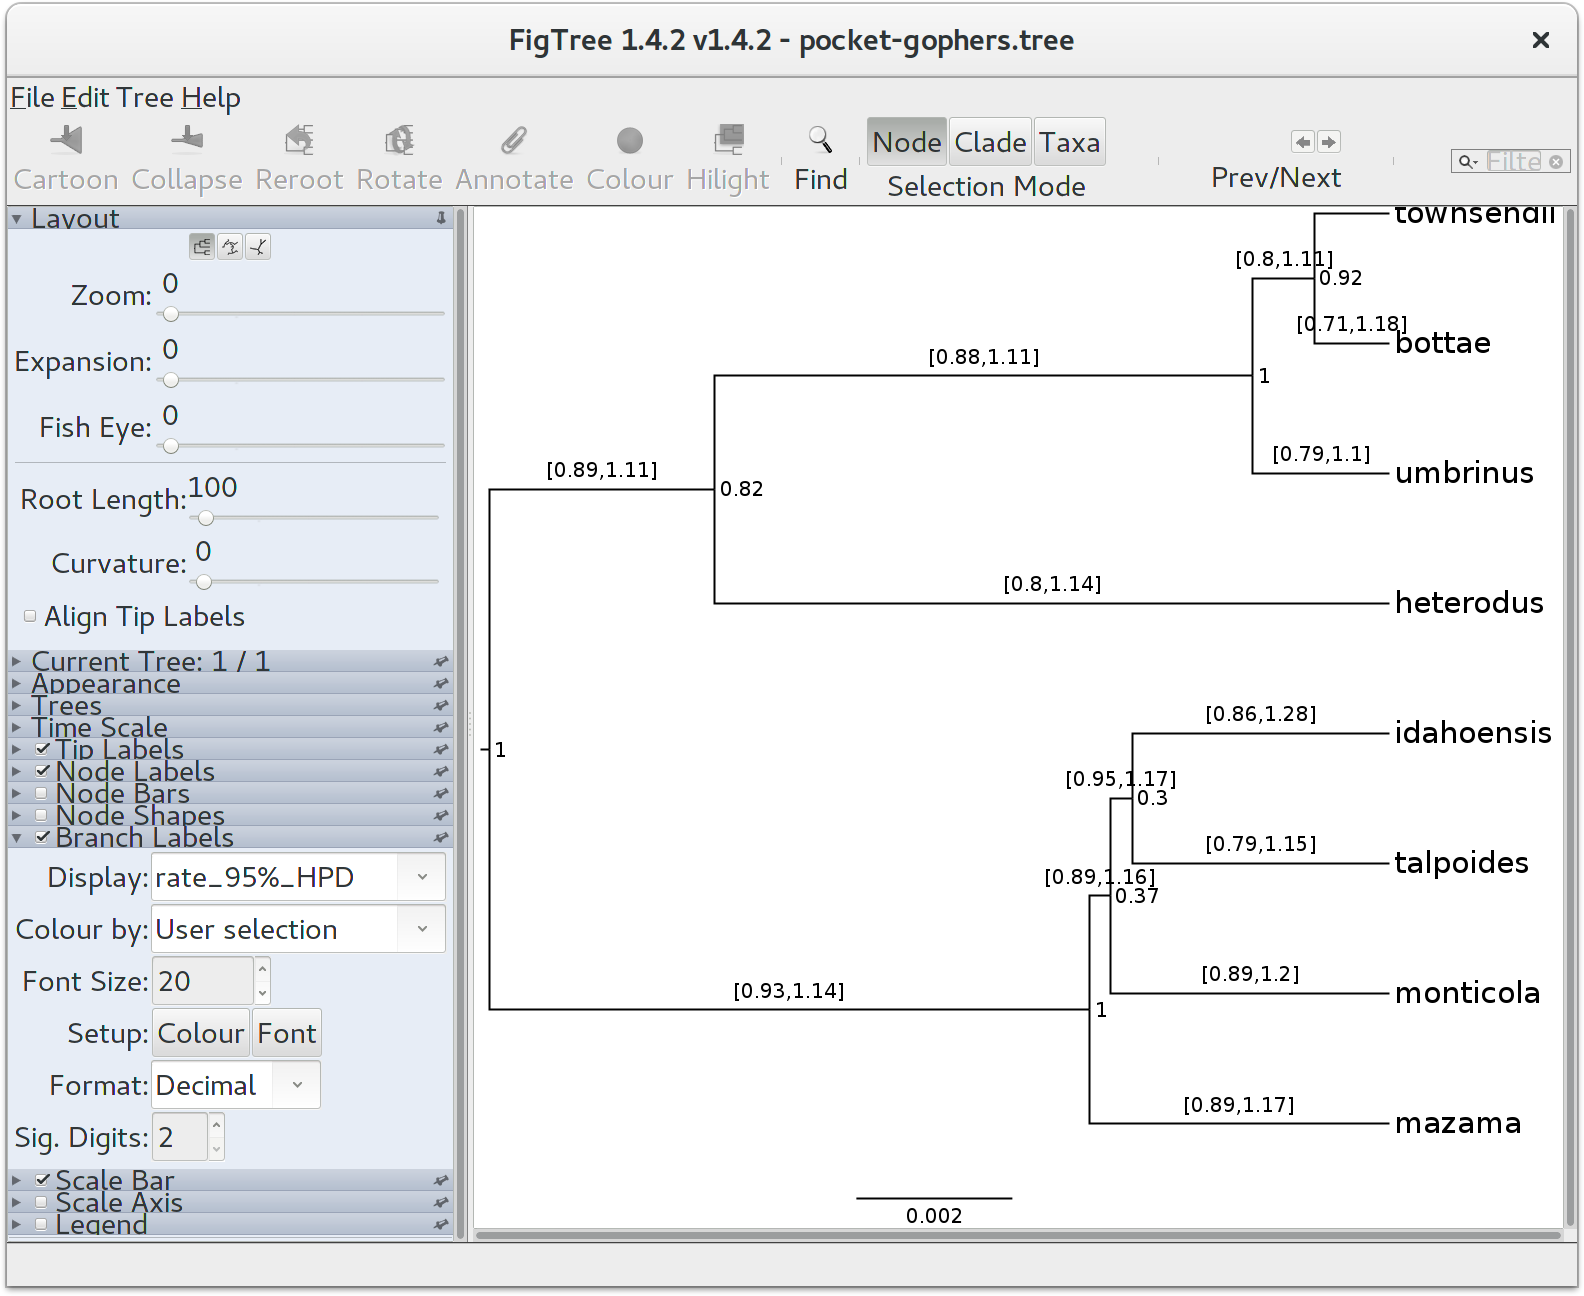
\includegraphics[width=\textwidth]{figures/figtree.png}
\caption{Figtree representation of the species tree.}
\label{fig:figtree}
\end{figure}

Notice that the HPD interval for per-species substitution rates all include
1.0, concordant with our previous observation that there may be no changes
to the overall substitution rate along this species tree.

As a more Bayesian alternative to FigTree, you can load the entire species tree
set into DensiTree. Open the ``species.trees'' file in DensiTree and set up the
cloudogram as follows:

\begin{itemize}
\item Select the \textbf{Central} geometry from the set of options in the top-right of the main screen.
\item Under \textbf{Show}, check the ``Root Canal'' tree to guide the eye.
\item Under \textbf{Clades}, check ``Show Clades'', display the means and 95\% HPDs using ``draw'', and display the posterior support
using ``text''.
\item Now, too many clades are shown, and most are not of interest. Check
``Selected only'', then open the clade toolbar using the \textbf{Window/View
clade toolbar} menu item. Select each clade (i.e.
items with more than one species) with majority posterior support (i.e.
with over 50\% support) by using the
shift key.
\end{itemize}

The image should look something like Figure \ref{fig:densitree}. Notice that
there is about 16\% support for \textit{heterodus} to be an outgroup, and about
82\% for heterodus to be in a clade with \textit{bottea}, \textit{umbinus} and
\textit{townsendii}. Can you explain where the remaining 2\% went?

\begin{figure}
\centering
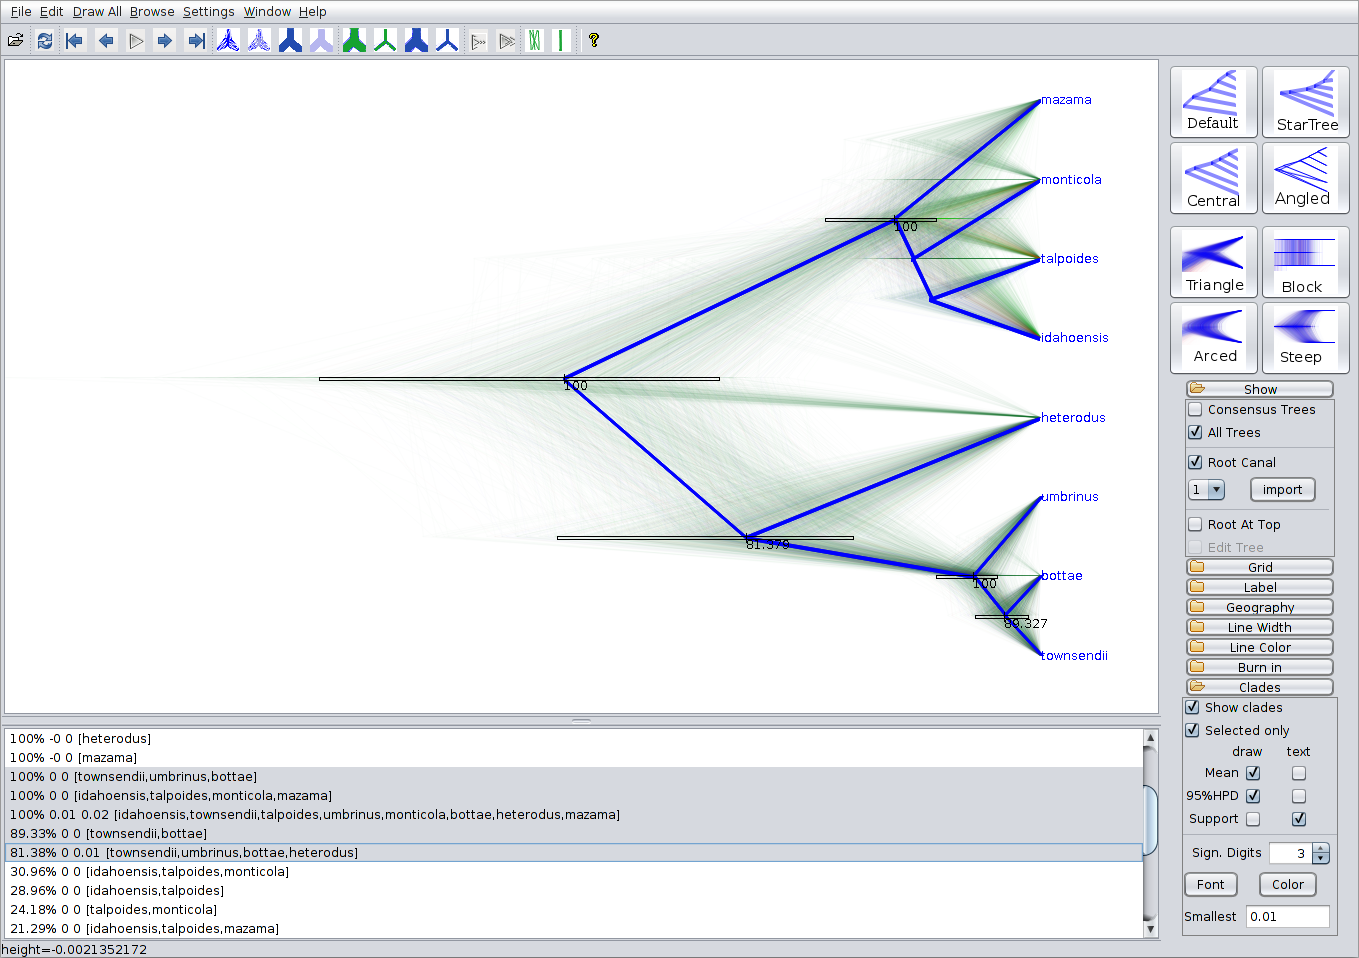
\includegraphics[width=\textwidth]{figures/densitree.png}
\caption{DensiTree representation of the species tree.}
\label{fig:densitree}
\end{figure}

\clearpage

\bibliographystyle{natbib}
\bibliography{StarBEAST2-tutorial-1}

\end{document}
